% !TeX root = ../main.tex
\chapter{Implementation}\label{chapter:Implementation}
As it mentioned in \ref{chapter:Background}, Carla simulator has been selected for our implementation.  In this work one of the built in maps of Carla has been used. In order to access Carla's assets like vehicles and maps, it provides a library which can be imported to python script and all we need as map(which is called World in Carla) and actors(or vehicles) and their properties are called through this library. First step of simulation was to define a favorite map which was suitable to our parallel parking project and spawn all vehicles in the map. As it has been already mentioned in the last chapters, this work is divided in 3 main steps:
\begin{itemize}
    \item \textbf{Detection phase}
    \item \textbf{Positioning phase}
    \item \textbf{Maneuvering phase}
\end{itemize}
The implementation process of each of them has been presented in the following sections.
\section{Detection Phase}
For the detection phase we used Matlab's tools and \acrlong{ml} libraries so it was also required to have access to Matlab and Matlab should be connected to Carla simulator. First the detection process in Matlab and then the method which have been used for Matlab-Python connection will be explained.
\subsection{Train ACF Detector}
As already mentioned in \ref{vehicle detection}, after comparing evaluation results of different detection methods, ACF(Aggregate Channel Features) algorithm has been chosen for the detection part. Before starting any detection, a detector is required so first step is to train ACF detector. we need to provide a dataset for the training step. Hence, different scans of vehicles in different locations and also in different orientations were provided. In this work about 150-200 images from all Carla vehicles were taken but before sending these data to training phase, Ground Truth objects should be defined in each image. Ground Truth object contains information about data source and list of all label definitions \cite{GroundTruth}. In other words all of images should be labeled in order to define ROI(Region Of Interest) to emphasize on object(here vehicle) which should be detected. For labeling Ground-Truth-Labeler application from Matlab \cite{gTruthLabbeler} has been used as it provides automatic labeling which makes a fast process and also it supports different image formats in various sizes and it is also possible to import unordered list of data to it. Figure \ref{fig:labeling} shows the environment of GroundTruthLabbeler and labeled vehicles using this application.
\begin{figure}
\centering
    \begin{tabular}{c|c}
         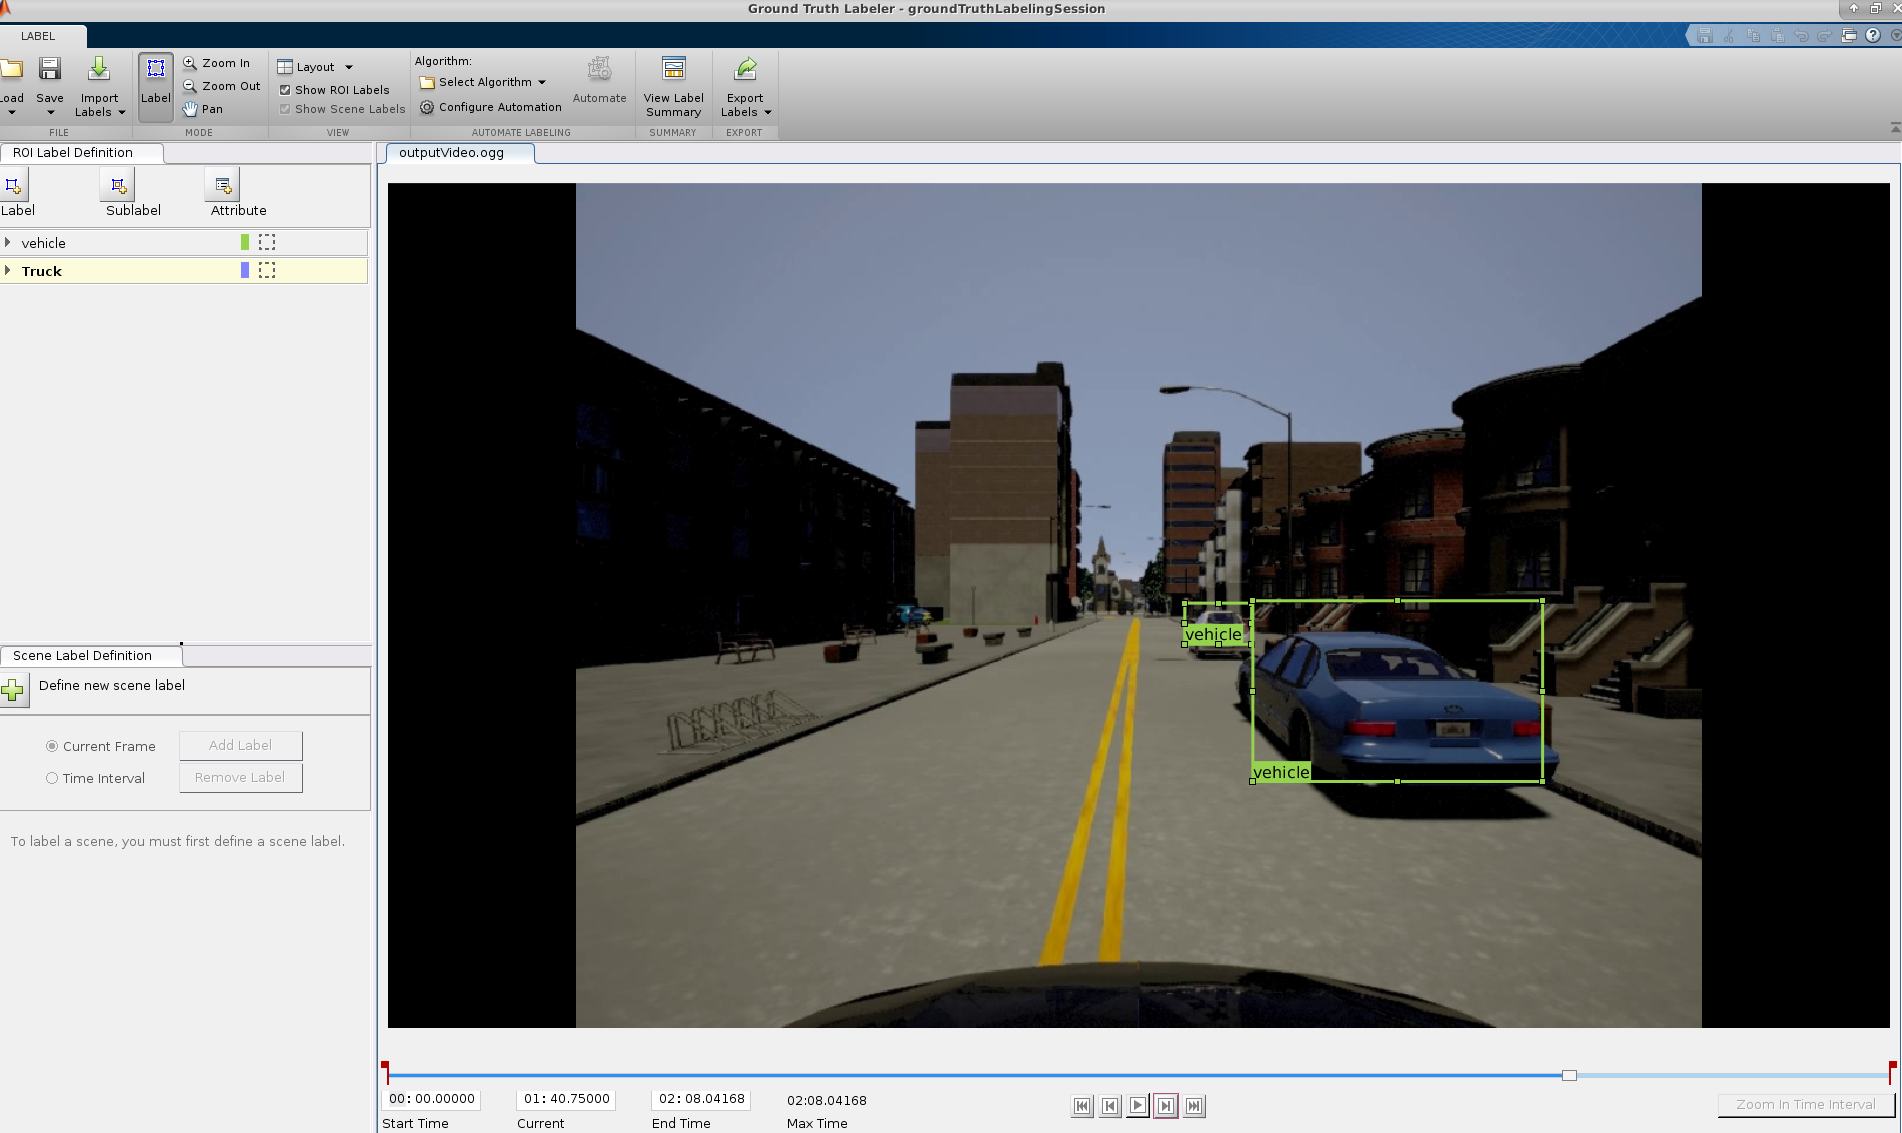
\includegraphics[width=7cm, height=6cm]{images/labeling1.png} 
         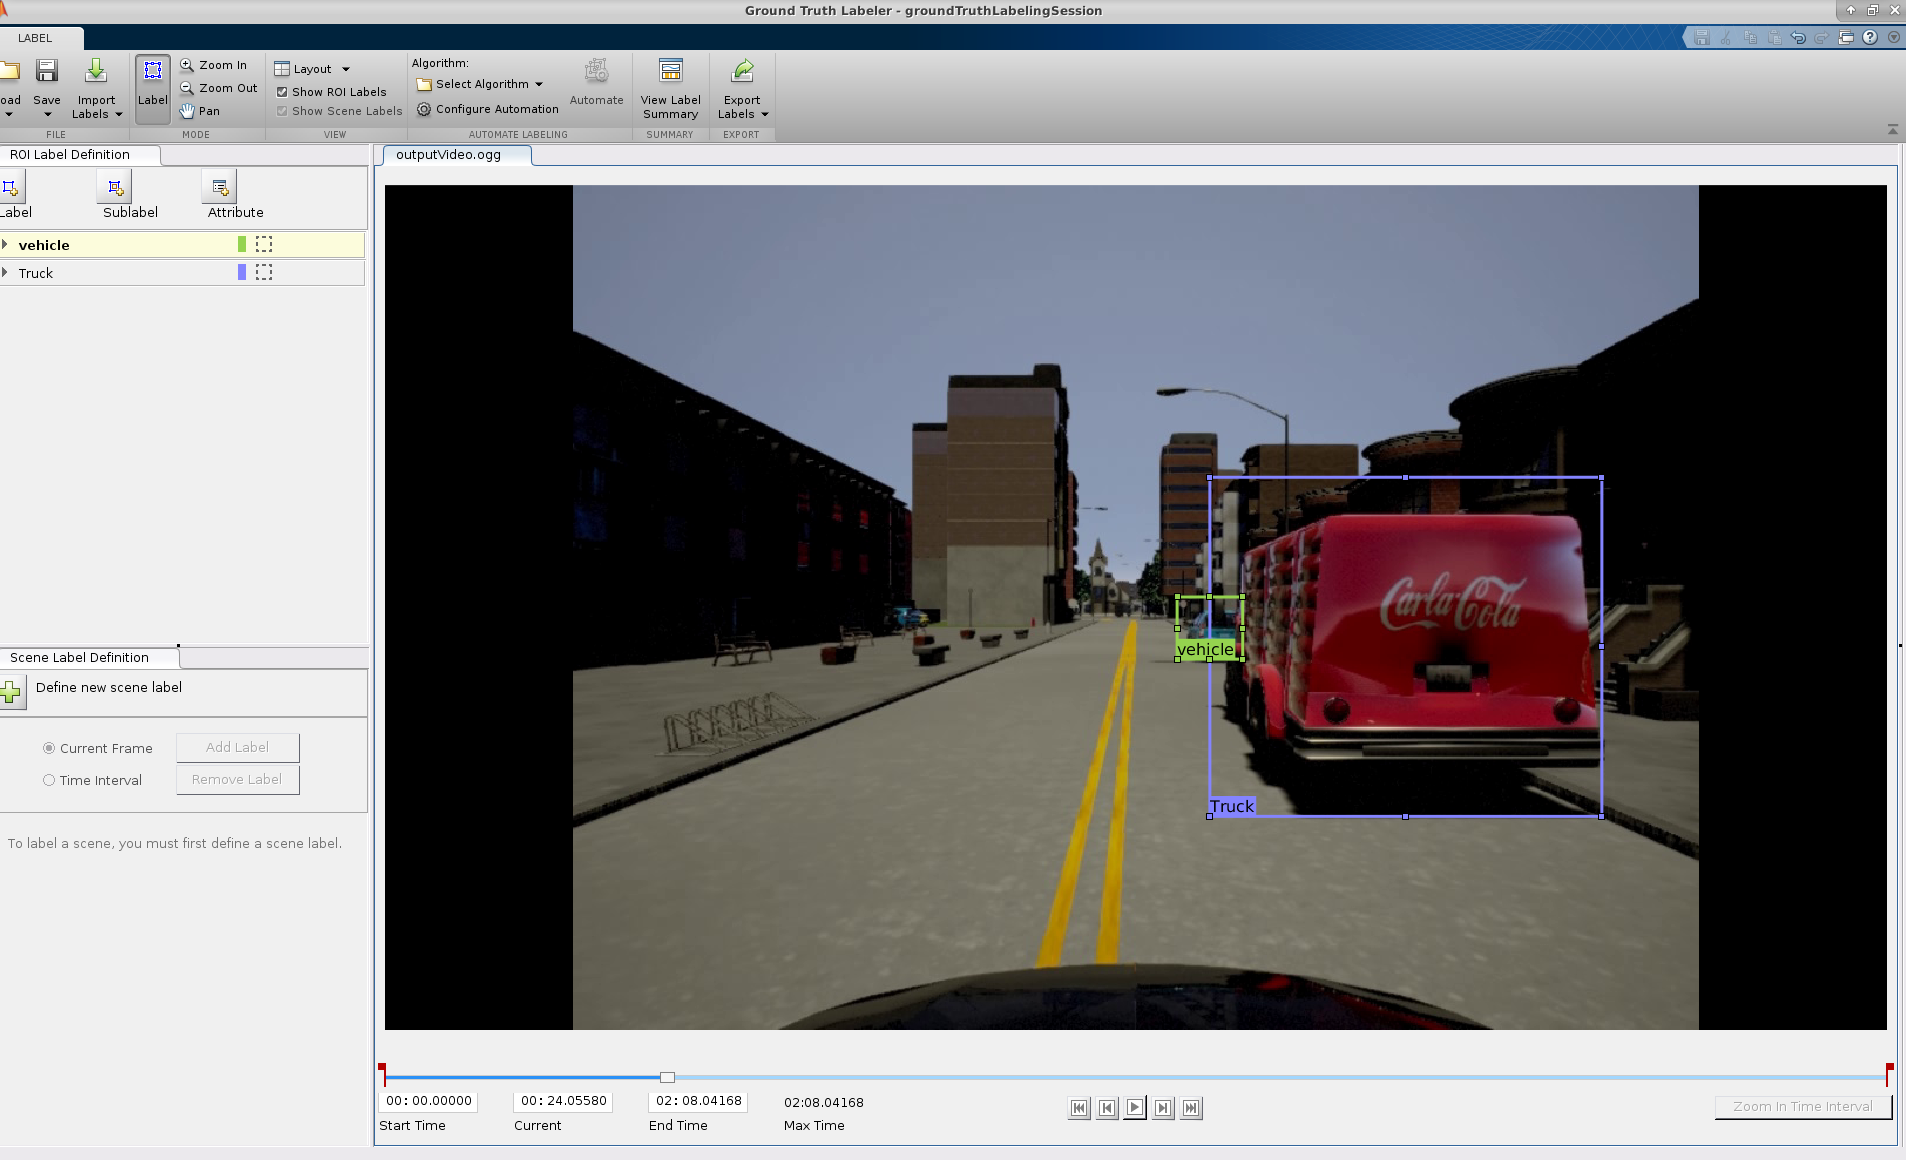
\includegraphics[width=7cm, height=6cm]{images/labeling2.png}
    \end{tabular}
    \caption{GrounTruthLabbeler Application}
    \label{fig:labeling}
\end{figure}

Training function of ACF library(called trainACFObjectDetector) has been used for learning phase and training property adjusted to 5 steps of training (5 is the empirical value that gave us a good result). \ref{fig:trainACF}shows the last step of training ACF detector.
\begin{figure}
\centering
    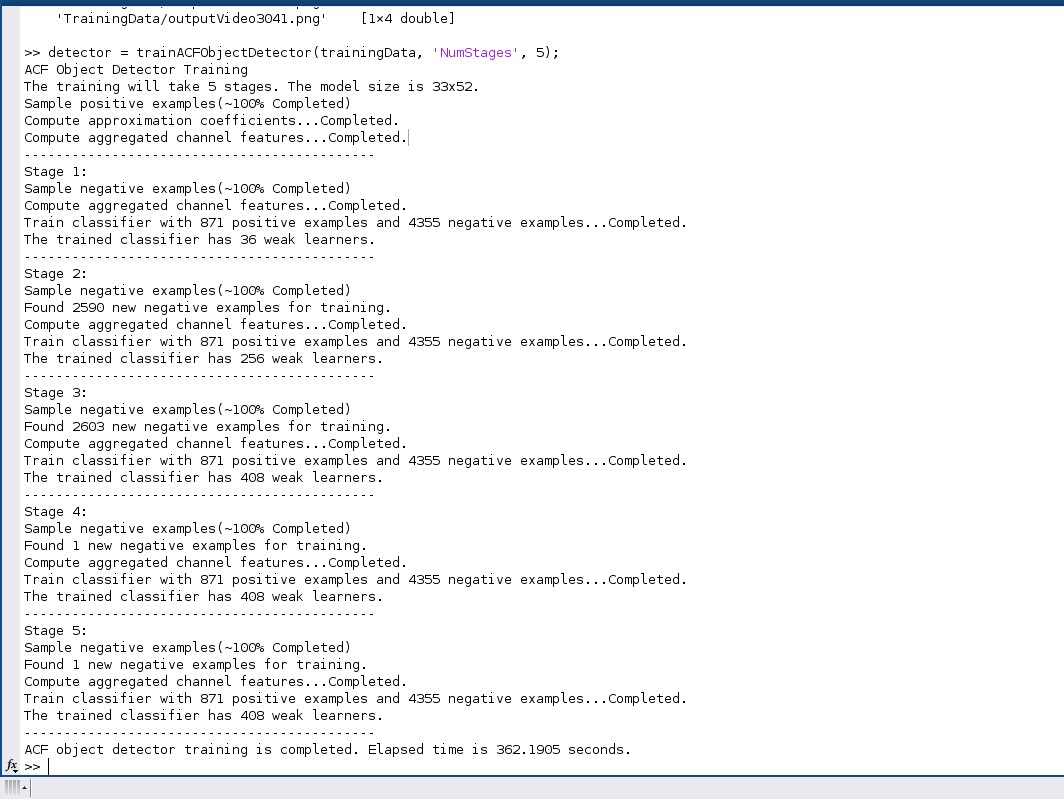
\includegraphics[width=12cm, height=7cm]{images/TrainpocessACF.jpg} 
    \caption{Training ACFObjectDetector}
    \label{fig:trainACF}
\end{figure}

After testing step, the detector was saved as it should be called for each time of running parking project. so second step was to test and evaluate the detector to guarantee that it will work in our parking project.
\subsection{Testing Detector} \label{test detector}
For testing the trained detector, a set of testing images which were not from training set, were selected. This images were labeled by GrounfTruthLabbeler to define the expected results. Raw images(testing set before labeling) were given to the detector in a for loop and detection results from all images were saved to a table. Finally, result table was compared to the expected results(labeled images) using evaluateDetectionPrecision function from Matlab. This function shows the rate of detection. As we have also seen the graph results of different detector in chapter \ref{chapter:Parking Space Detection}, ACFObjectDetector had the best rate in out data.(70 percent accuracy)
\subsection{vehicle Detection} \label{car detection}
The tested detector \ref{test detector} is called whenever we run the program and before start of parking maneuver to find a parking vacancy by using detect() function of ACF library. This function gets an image as input argument and compares it with the detector and its outputs are scores and bboxes' coordinates. 
\begin{figure}
    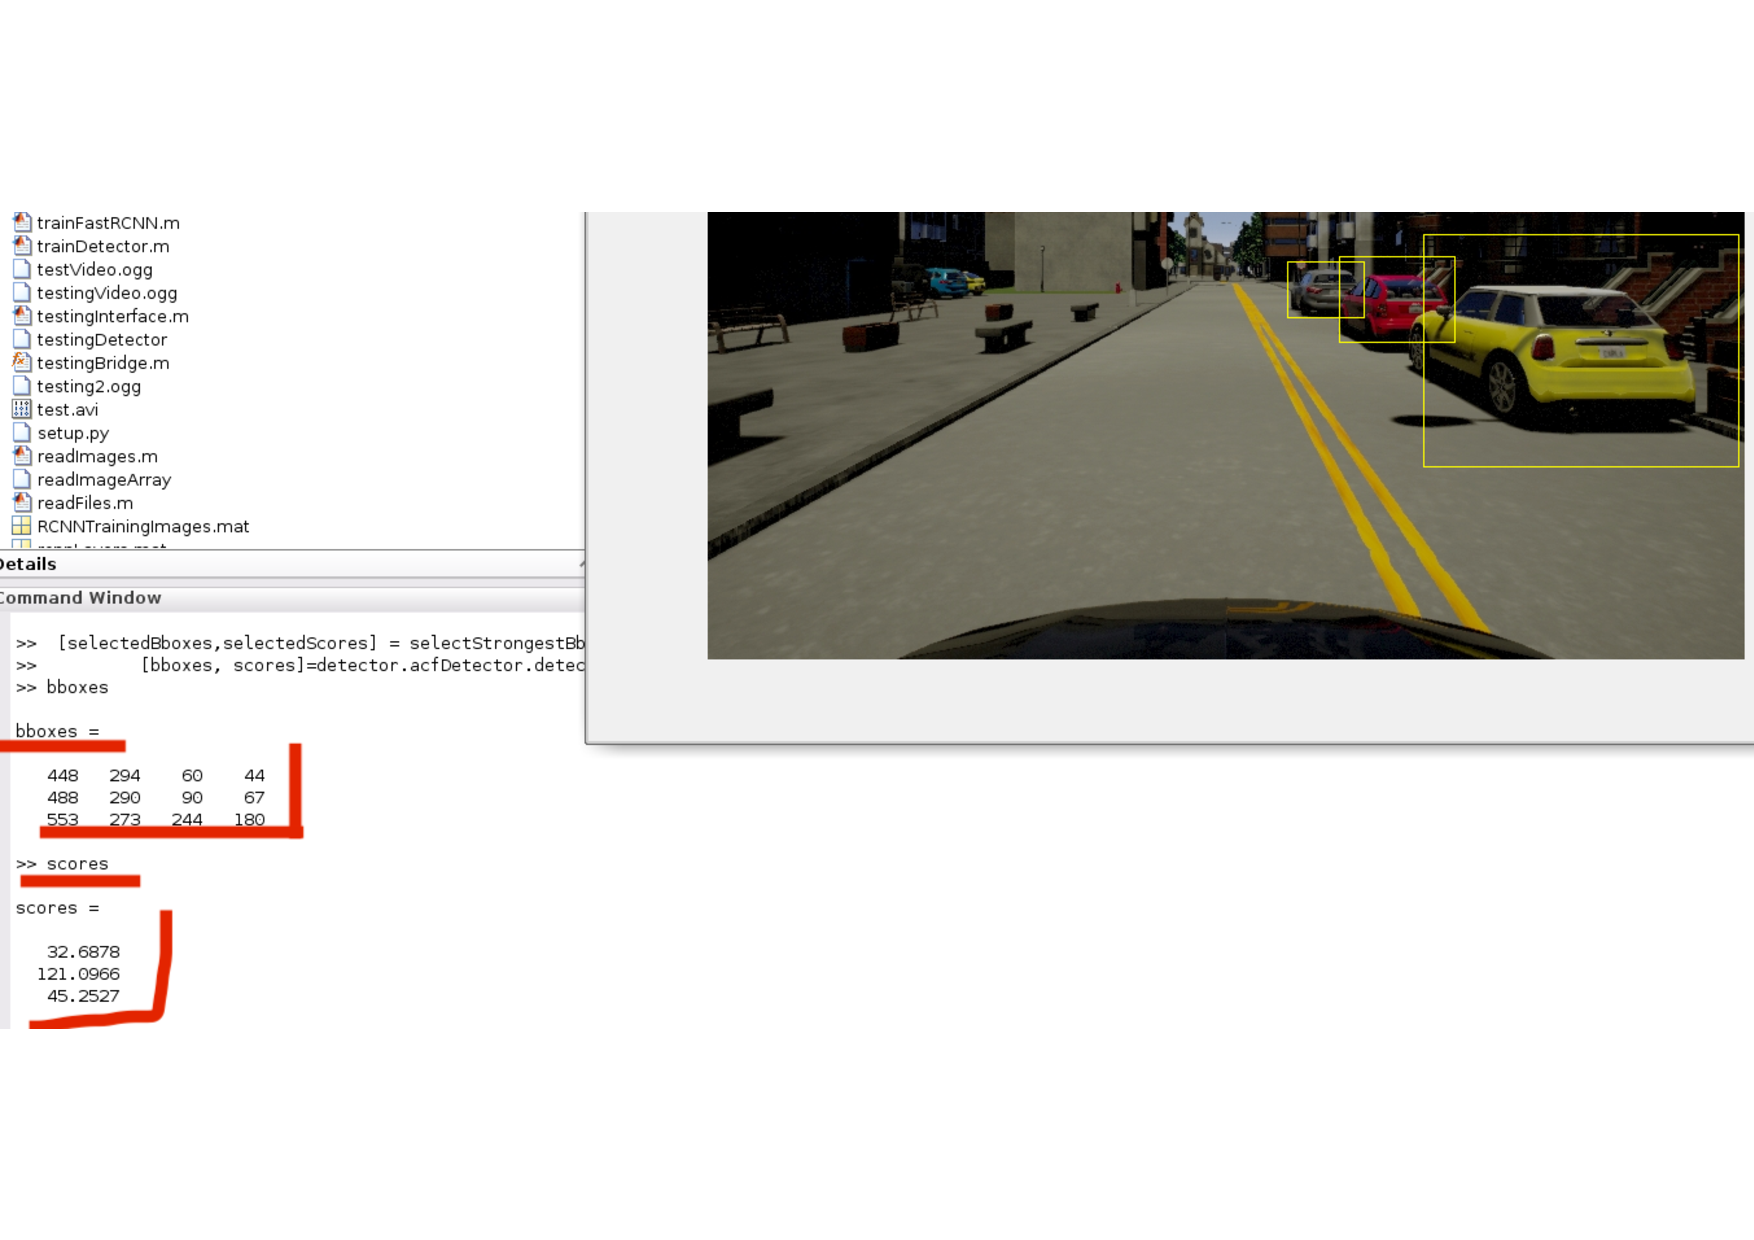
\includegraphics[width=12cm, height=8cm]{images/bboxesAndScores.pdf} 
    \caption{Results of ACF Detector-\acrfull{bbox} and Scores}
    \label{fig:BboxesAndScores}
\end{figure}

Fig \ref{fig:BboxesAndScores} illustrates an example of applying ACFObjectDetector on a test image. As it can be seen the results are shown as Scores and \acrshort{bbox}. Scores refer to the detection score or rate of detection in percentage. \acrshort{bbox} shows the place of detected vehicle and also height and width of the box surrounding vehicle. \acrshort{bbox} can be defined as [x, y, width, height]. we used these values to estimate size of the vehicle. In order to see bboxes around the vehicles, Matlab's annotation function of Image processing toolbox could be used. After applying annotation function to image, bboxes will be added to image so detected vehicles would be covered by boxes around them fig \ref{fig:detectionSamples}
\begin{figure}
\centering
    \begin{tabular}{c|c|c}
         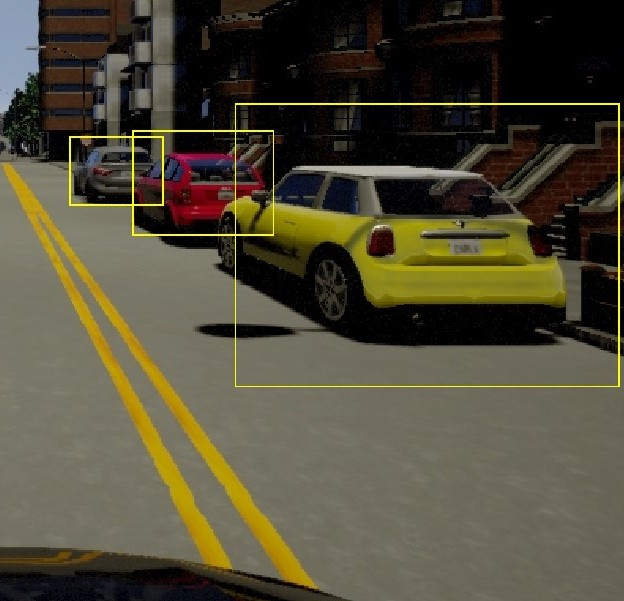
\includegraphics[width=7cm, height=5cm]{images/acf.jpg} 
         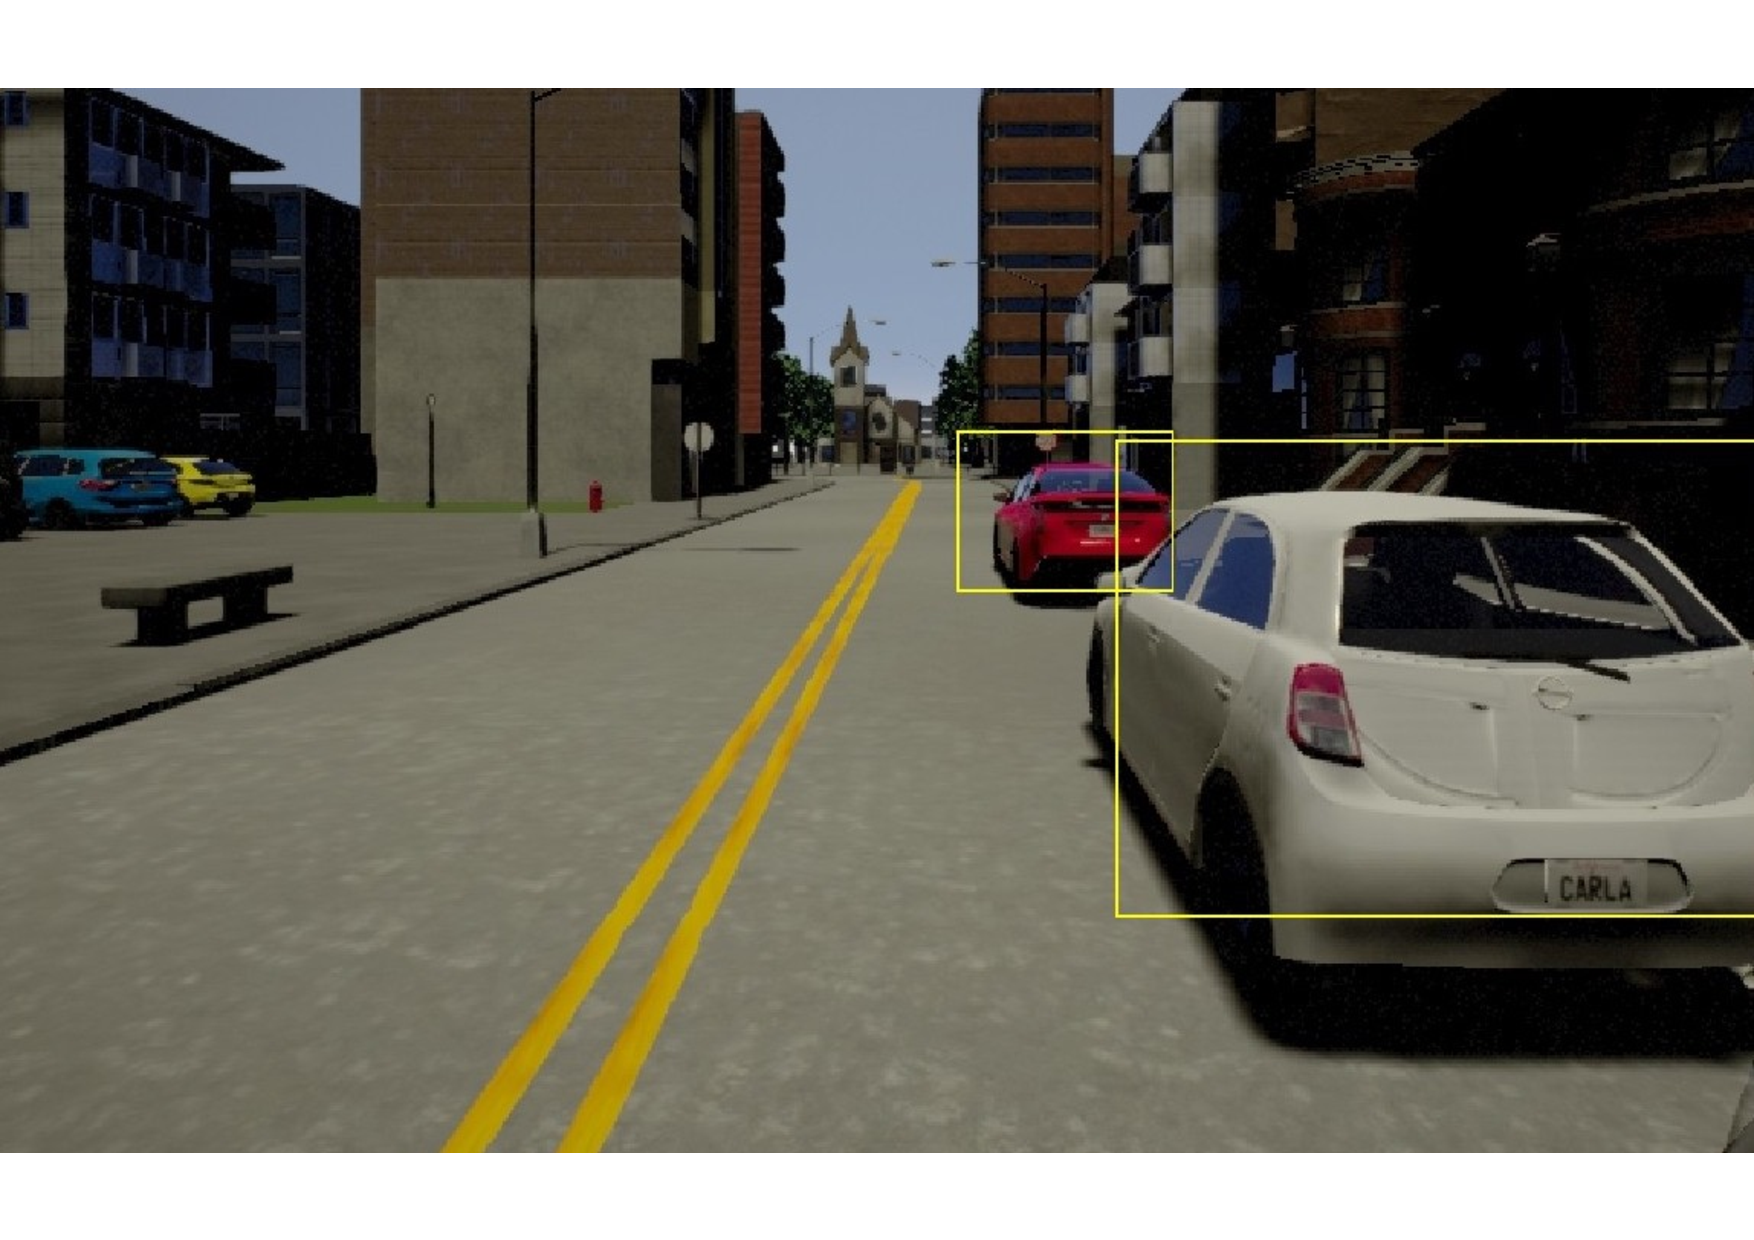
\includegraphics[width=7cm, height=5cm]{images/test4ACFview.pdf}
         %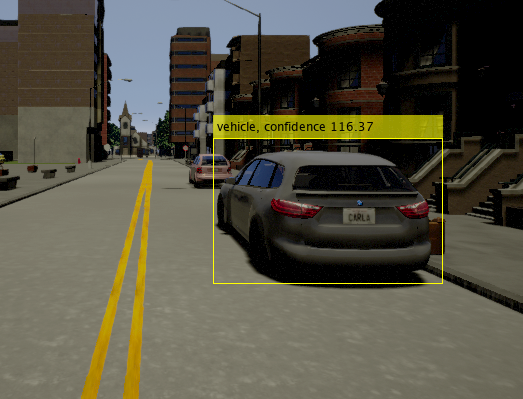
\includegraphics[width=4cm, height=6cm]{images/detection.png}

    \end{tabular}
    \caption{Detected Vehicles}
    \label{fig:detectionSamples}
\end{figure}
\subsection{parking vacancy detection}
As it has been explained in \ref{chapter:Parking Space Detection} to estimate the place of parking vacancy, bounding boxes are used to find empty parking place. However, before calculating the overlap ratio, we should select bboxes with the strongest detection rate(strong scores). Another problem is that in some cases there are multiple bboxes for one detected vehicle with different detection scores. So if there would be multiple bboxes for one vehicle, \acrshort{bbox} with the highest scores should be selected. After selection of the strongest boxes, each of the vehicles in front of the ego vehicle would have one bbox covering them, as we could see in fig \ref{fig:detectionSamples} from detection results, this bboxes have overlaps. In this work, we use these overlaps as a criteria to discover parking vacancy. If the rate of overlap is very small, it means that two adjacent vehicle are far from each other so there is enough place for parking between the. However, when this ratio is high it means that two vehicles are closed and there is no other space for a new car between them. Here overlap rates were calculated by using Matlab bboxOverlapRatio function. When this ratio is smaller than the threshold, it could be ignored so there could be a parking spot between 2 vehicles. Here, searching for parking place would be stopped and the area of detected parking place would be calculated by sensor and compared with vehicle's size to make sure that it is a suitable place for parking. 
\subsection{Connect Matlab to Python-API}
In order to access our trained detector during simulation and find parking place, Matlab should be connected to Carla because the default API in Carla is python so we should have made a bridge between python-API(which is directly connected to Carla) and our Matlab codes(to access detector and detection libraries in Matlab). Figure \ref{fig:python-matlab} illustrate interface and the steps for connecting Matlab to Python.
\begin{figure}
    \centering
    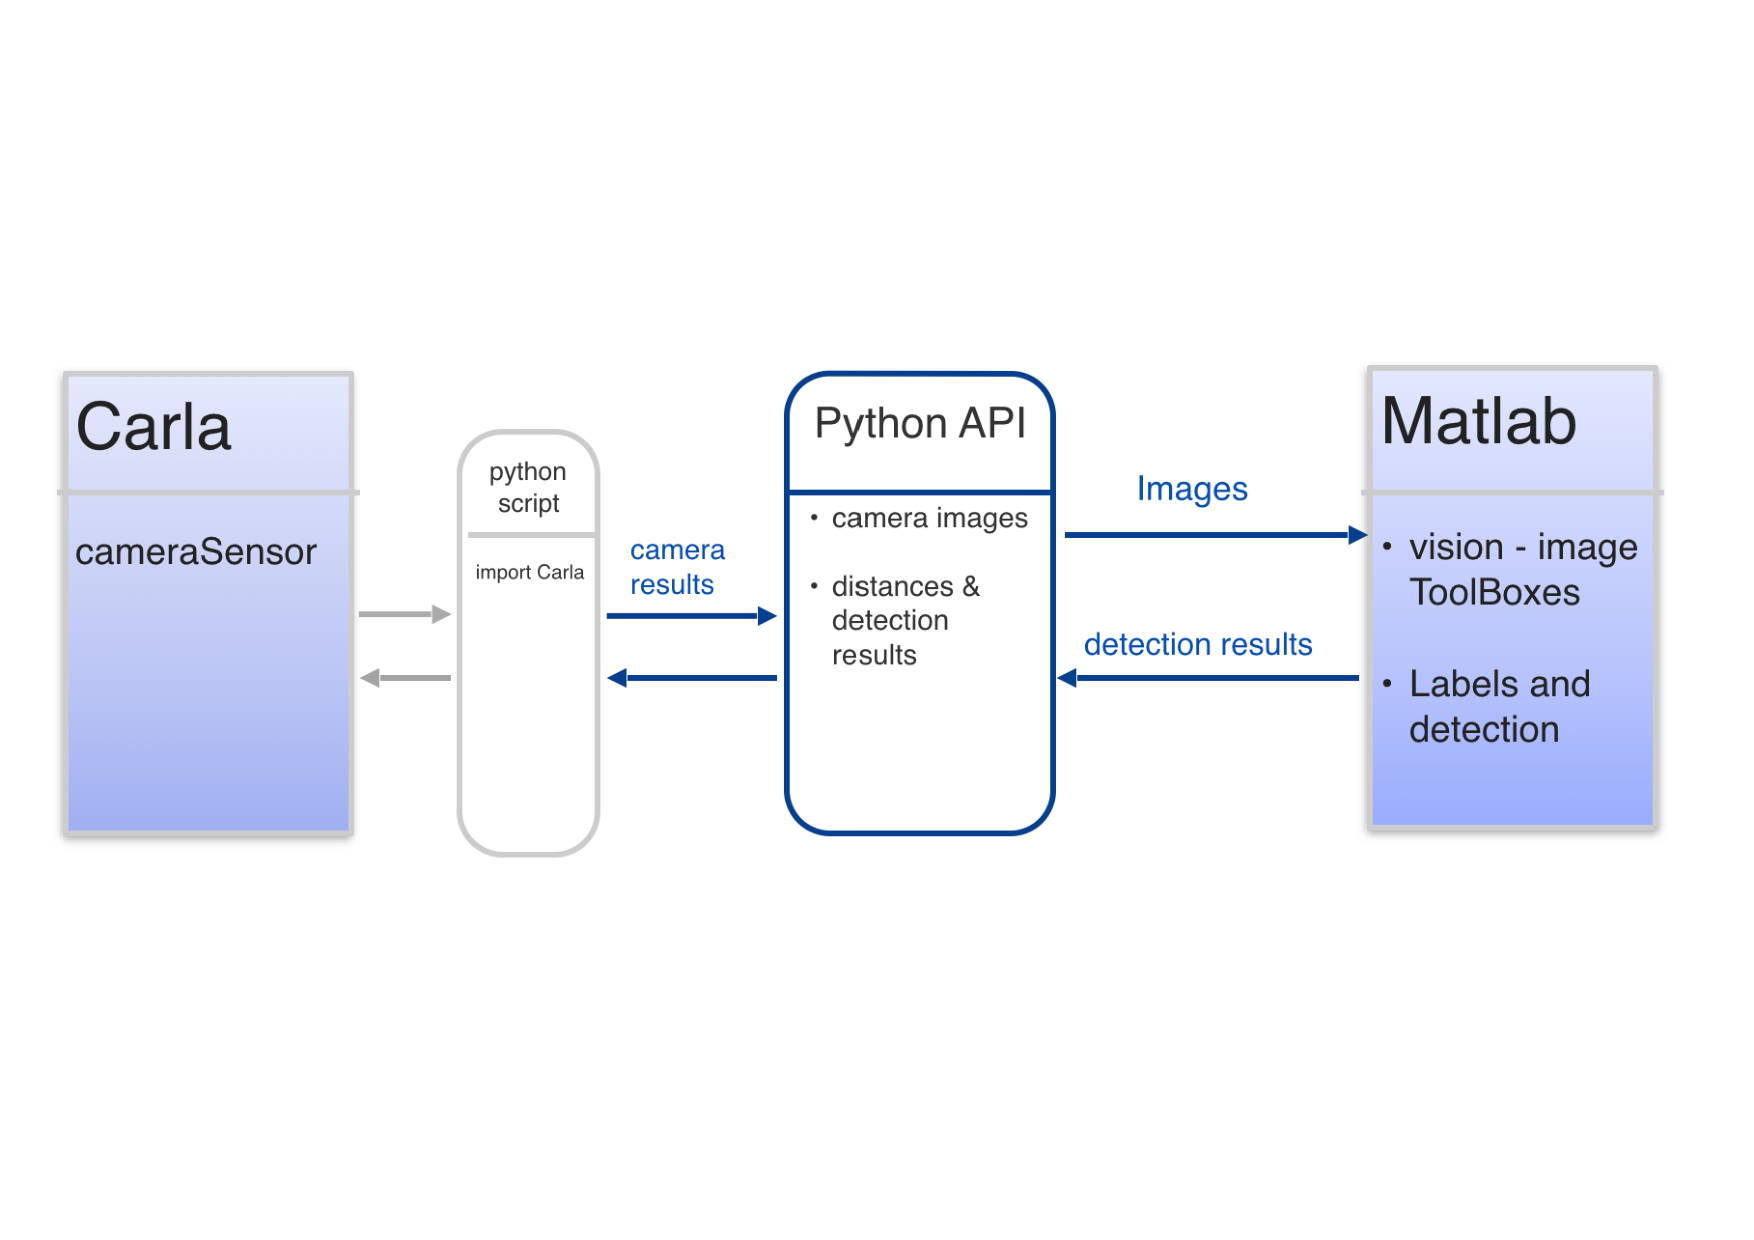
\includegraphics[width=12cm, height=6cm]{images/carla-matlab.pdf}
    \caption{Python-Matlab connection}
    \label{fig:python-matlab}
\end{figure}



Various methods and libraries has been defined in recent years either by Matlab and Python developers. In this work at first we decided to use MatlabEngine library which is offered by Matlab \cite{matlabEngine}. Matlab-engine provides different methods to read data from Matlab to python and vise versa. At first there were some settings in python and Matlab before using it as it should be installed in both sides (python and Matlab) and import to their libraries. However, this method was not successful for us because what we wanted to import from Matlab to python was our trained detector and the format of detector was not supported by Matlab engine. Detector type is specific type of double struct in Matlab and as it can be seen from type mapping table provided by Matlab \cite{matlabEngineFormats}, struct type always translated to dict type in python and when detector was translated to dict type, everything were disturbed in that as we could not get the bounding boxes and scores and also was not possible to access detector's parameters and functions for detection in that format. So other ways of connection should have been tested. There are also different tools offered by python as Numpy/Scipy libraries offered different tools for this goal. After testing different methods, finally what is offered by pymatlab \cite{pypi} has been selected which was the fast way of connection and it also support different data types from Matlab. The good point is that we could access to the whole .m file at once without need of going through Matlab codes and read each variable separately. That is really straight forward where pymatbridge installed once and could be imported to our python files to access all of the .m file. Fig \ref{fig:interface} shows the interface function for calling parking.m file from Matlab in PythonAPI. File parking.m includes detection function in Matlab which calls ACFDetector and calculate the detection results.
\begin{figure}
\centering
    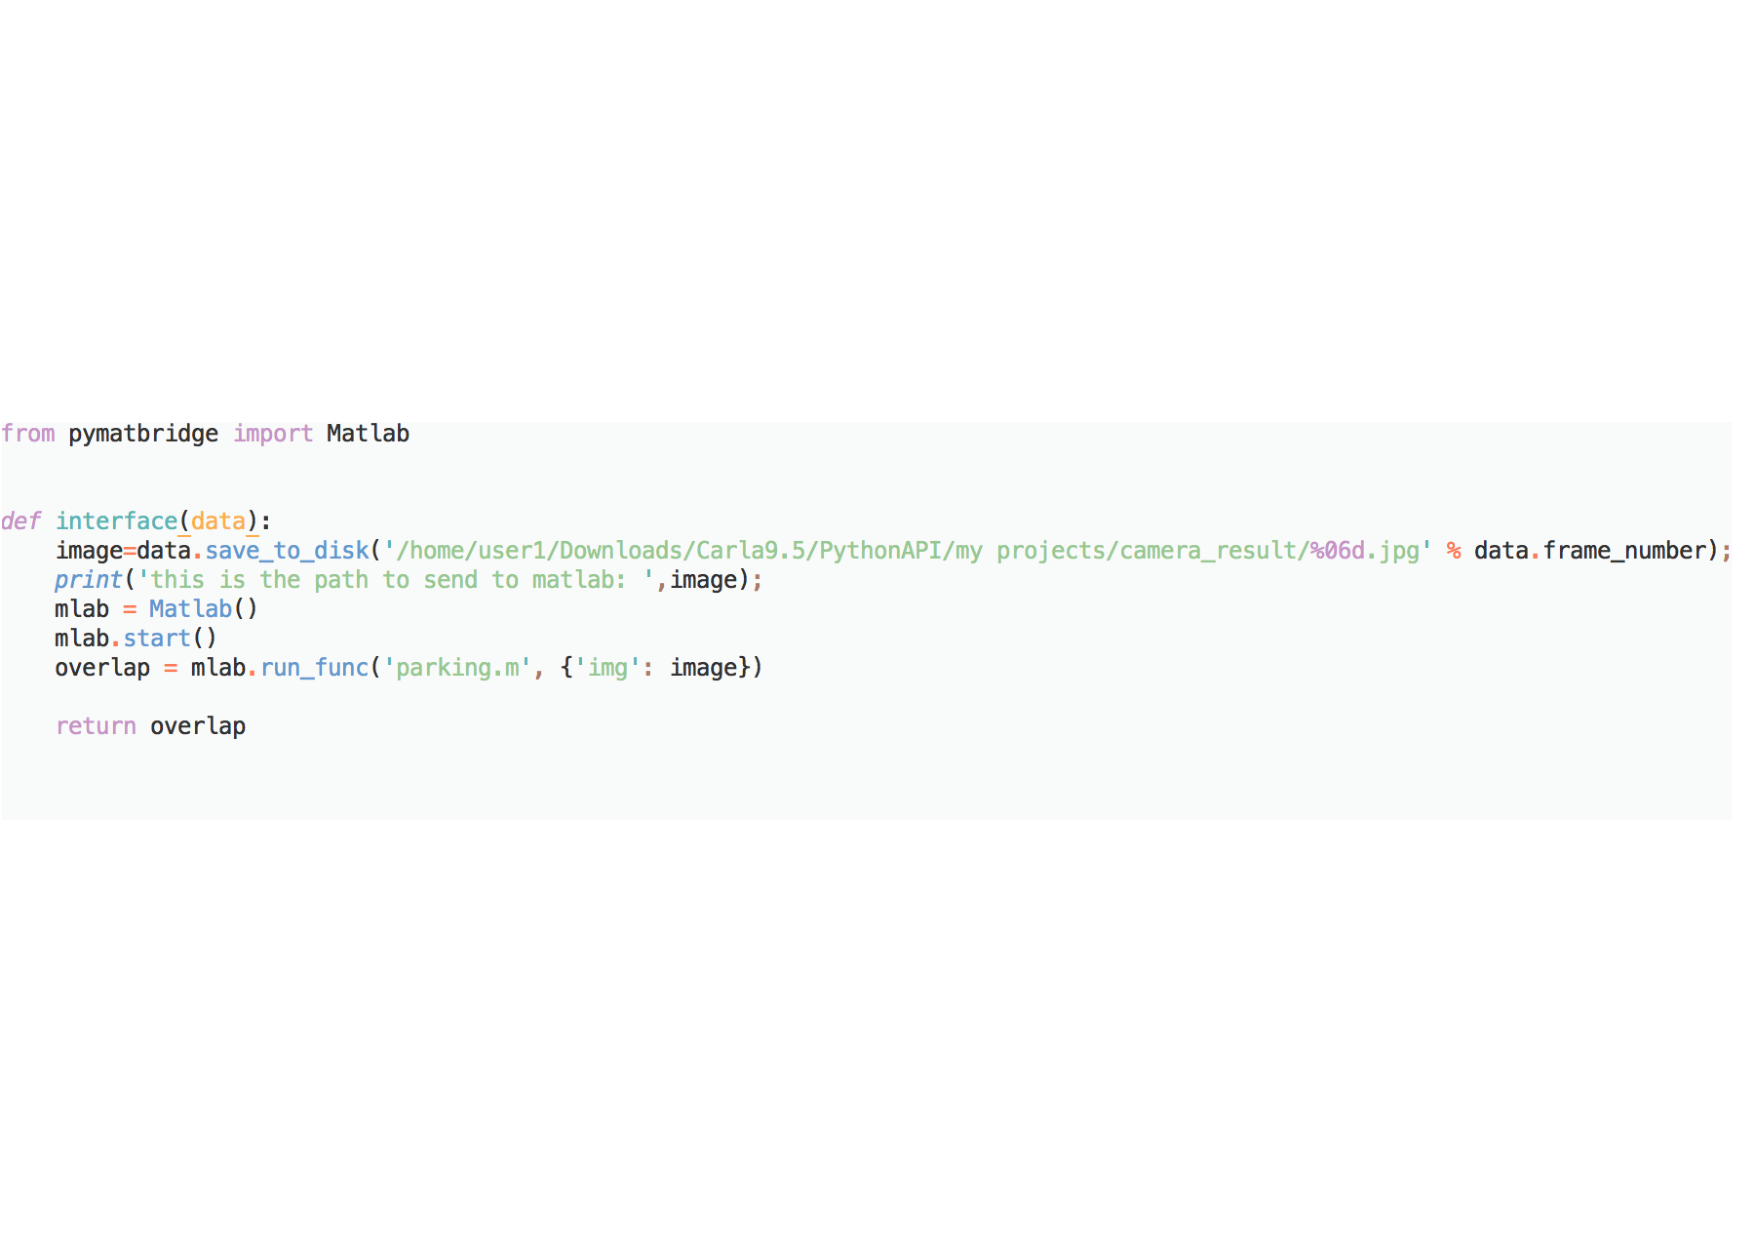
\includegraphics[width=12cm, height=6cm]{images/interface.pdf}
    \caption{Call Matlab file from Python}
    \label{fig:interface}
\end{figure}


According to \ref{car detection} section, to detect vehicles and find parking place we need to get an image of the vehicles and send it to detect() function in Matlab to compare it with detector. As we need image data for detection, we used a camera sensor which is attached to the ego vehicle and provides image files to send to Matlab.

\subsubsection{Camera sensor}
Camera sensor is placed in front of the ego vehicle and in each capture, its output which is an image file will be sent to .m file (Matlab) to find the parking vacancy. The idea is that in each tick or capture of the sensor, vehicle is stopped from moving and also camera sensor is stopped and wait for the result of Matlab file to see if the parking place is detected or not. If the parking place is there, camera sensor will be stayed deactivated and we will go to maneuvering step. Otherwise, it camera-sensor turned on again and vehicle set to continue to its forward moving and again by another capture, last process repeated again till a parking place would be detected. The codes for detection part and analyzing camera data are written in parking-decision function and can be seen in Fig \ref{fig:camera}. This code will be executed each time camera sensor provides a new data (image file) and is an iterative process till the detection of parking place.
\begin{figure}
\centering
    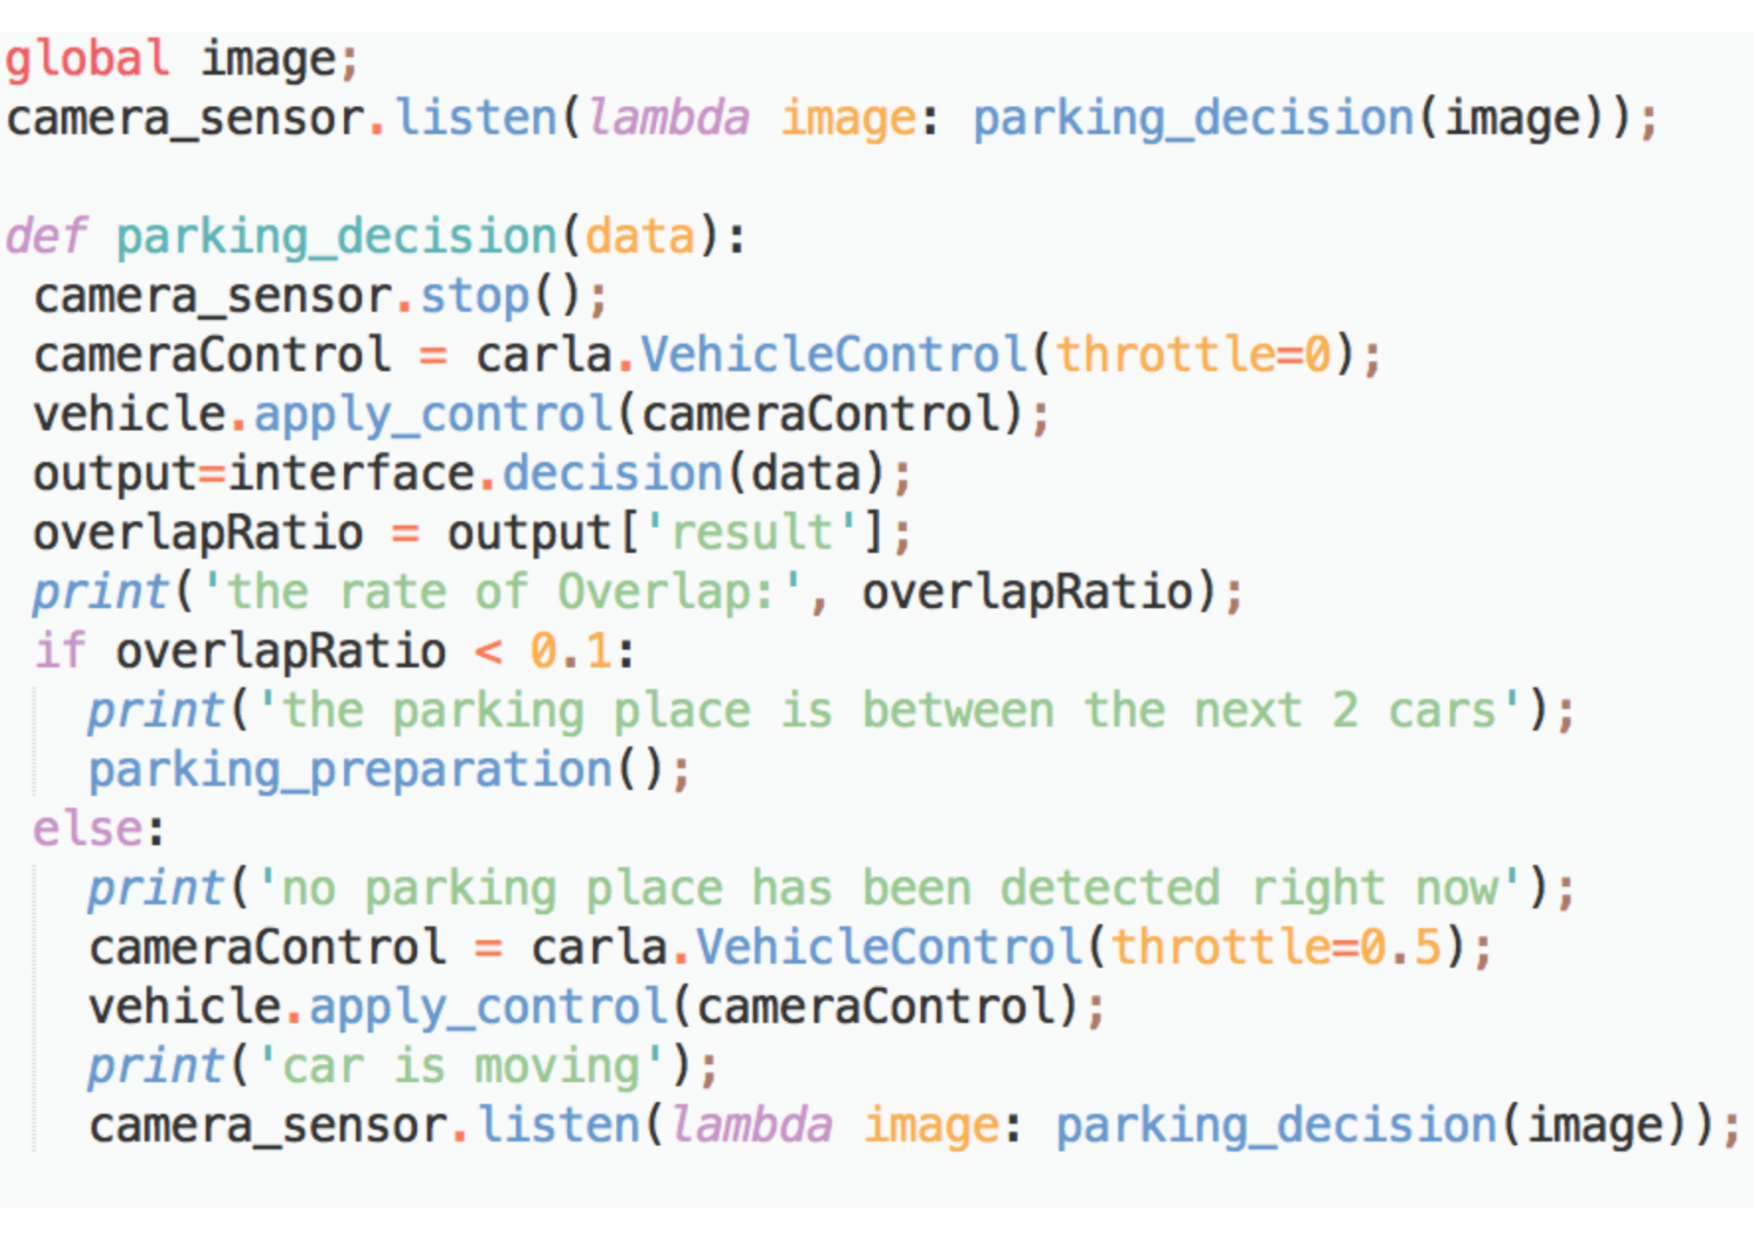
\includegraphics[width=10cm, height=6cm]{images/cameraSensor.pdf} 
    \caption{Camera-Sensor}
    \label{fig:camera}
\end{figure}

The idea of deactivating camera sensor after each capture is to wait for the .m file or Matlab's result after each time of capturing. so it will makes a synchronization between Matlab and python. python is always faster than Matlab and that is also because of the process is done by Matlab as reading all detection libraries and comparing to the whole trained data in detector takes more time of process. so in order to sync the process, vehicle and sensor will be deactivated. Otherwise, if there would be no synchronization, vehicle continue its movement and camera sensor generates other photos and send them to Matlab while the process of last image in Matlab has been not finished yet. so many of output images from camera would be dropped and will not processed in Matlab even if they may contain important information. Also if vehicle continue to its movement while  Matlab is in the process it may finished the path and passed through all vehicles and parking place while no photos has been sent during its movement and .m file is still processing last result. As there might be many repetitive photos in camera-sensor's result, it has been set to get photo in every 5 second instead of every second because in that way there would be many redundancy where many same JPEG files would be sent to .m file that makes the program really slow.
As it has been seen in \ref{fig:camera}, overlap ratio is returned from  Matlab as a result of detection in each sent image. Here this rate is compared with the threshold of 0.1(empirical value). If the overlap rate is less than threshold, the space between two vehicles ahead will be considered as a parking-bay. 

\section{Positioning phase}
After detecting parking place, vehicle should be set to the start position for parking. we know that parking place is between the next two cars so the ego vehicle should pass these cars and stop beside the second car(parallel to that) to start a reverse movement to the parking vacancy. 
As already mentioned in \ref{chapter: stabilization} chapter, longitudinal and lateral displacement of the parking-bay should be also measured and this values should be compared to the ego vehicle's size to ensure that this is a right parking place where vehicle would have a safe movement without collision. Besides, these data will be also needed to implement maneuver algorithm in the next step. For the measurement of parking area, also distance to the obstacles and detection of other cars Obstacle-sensor of Carla has been used. As we have seen in \ref{fig:sensorPlaces}, three sensors have been placed in the right side of the vehicle because parking place in our environment is in the right direction and one sensor the rear of vehicle car is for controlling distance to adjacent vehicles and ensure collision-free maneuver.
Sensor in the center of right side of the vehicle is for detection of other vehicles. During stabilization phase, vehicle moves slowly in the left side of the parked vehicles and results from the sensor are read. we used a counter to record number of detected vehicles by the sensor when the counter comes to 3, it means that vehicles should be stopped and this sensor will be stopped. Why this is 3? because at start point where we get the result of Matlab detection, vehicle is located in the side of a non-player where stabilization phase is started. This non-player was not in the last image of camera sensor where parking vacancy detected but when vehicle starts to move this non-player will be also detected by obstacle sensor so counter will be also increase by that detection at start of the movement. Counter should become to 3 means that vehicle has passed 2 vehicles in front besides the first one at the start of moving. To find longitudinal displacement of parking bay, sensor locations after passing the first vehicle(counter=2) and in start of detection of second vehicle(right after counter becomes 3) will be recorded. Distance of these 2 locations is longitudinal displacement of parking-bay. 
when second vehicle is detected, vehicle should be stopped moving. In this step distances of 3 right sensors to the parked vehicle should have the same value to ensure that vehicle is in parallel to the parked car. The codes for this step has been written in a function called parking-preparation as it can be seen in fig \ref{fig:position}.
\begin{figure}
\centering
    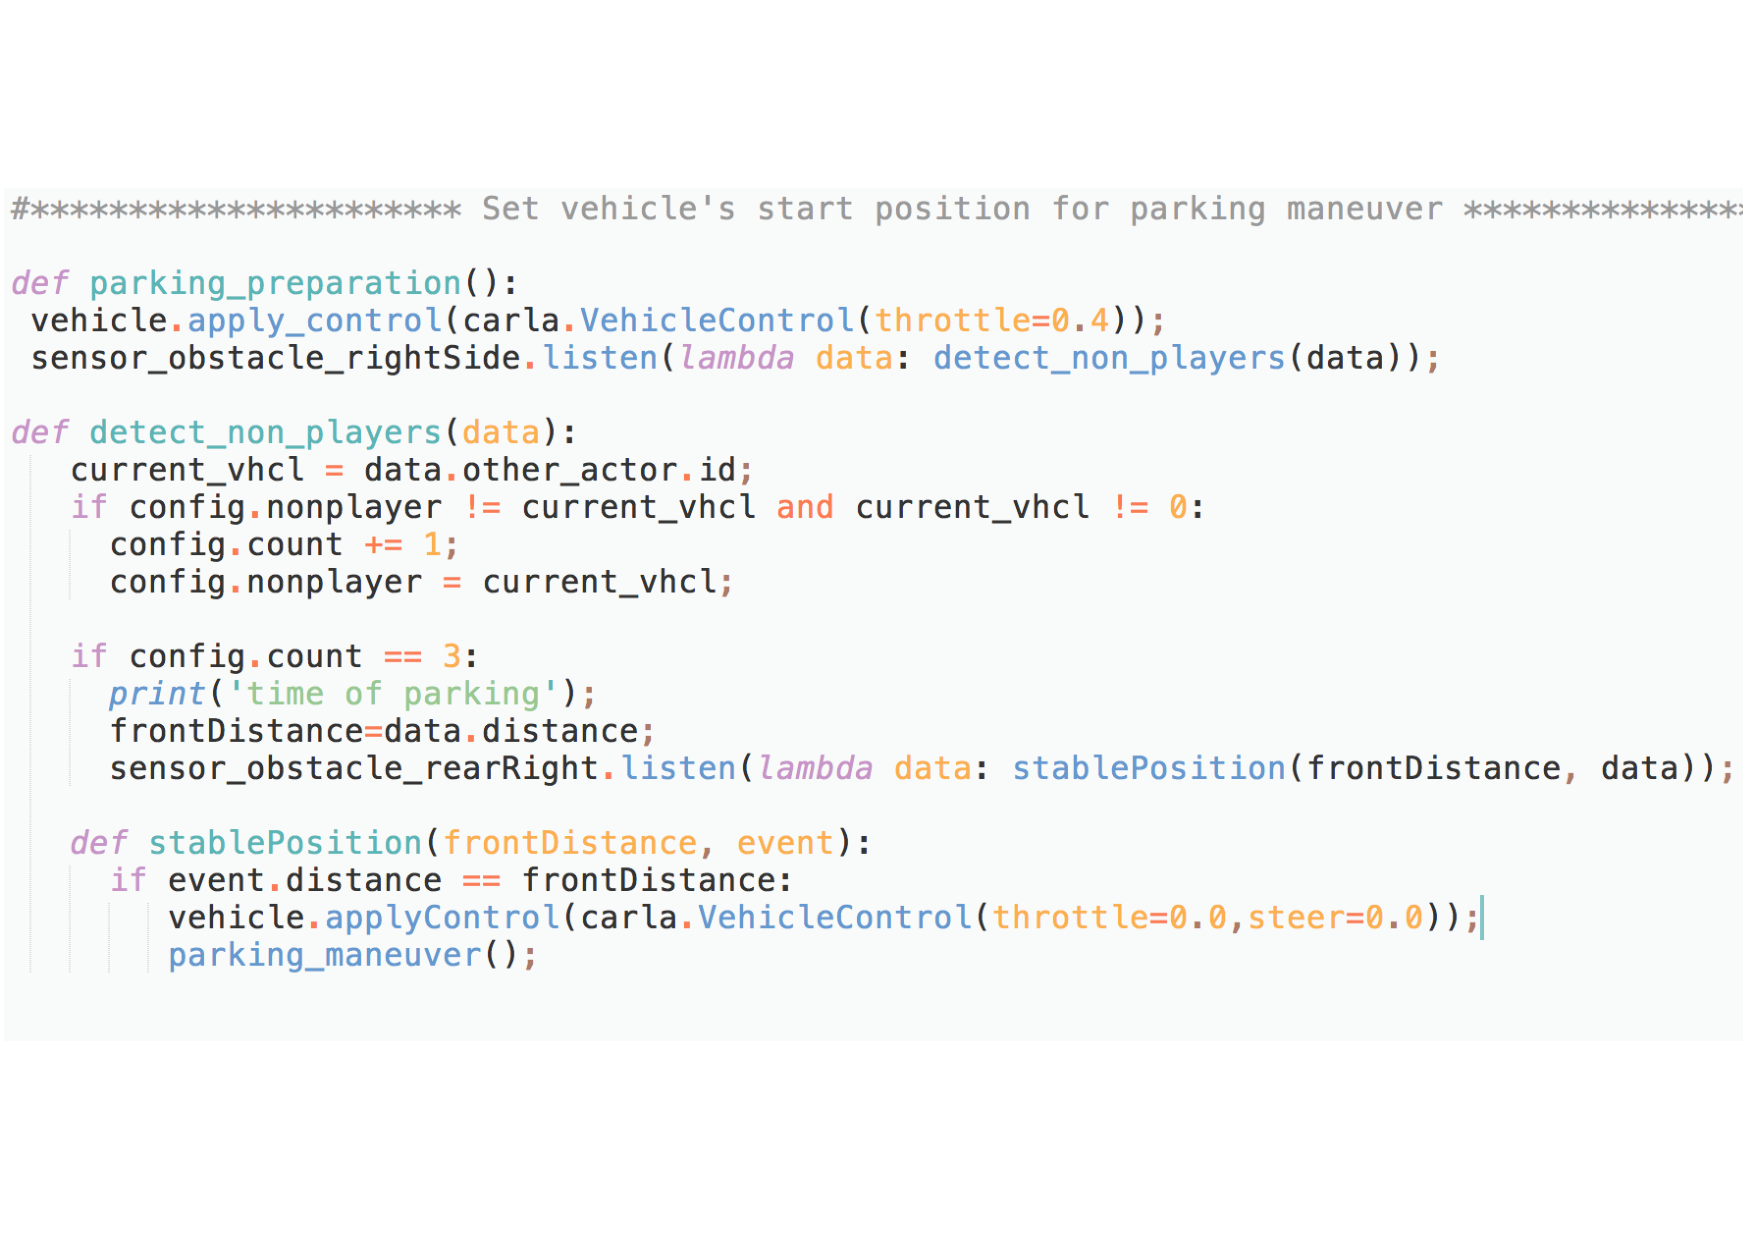
\includegraphics[width=12cm, height=6cm]{images/positioning.pdf}
    \caption{Parking-preparation}
    \label{fig:position}
\end{figure}

\section{Maneuvering Phase}
Implementation of this phase realizes the concepts presented in chapter \ref{chapter:Parking Maneuver}. All of the implementation codes has been written in python using python mathematical tools and numpy libraries. Calculation of steering angle, time and velocity has been written in maneuver.py file which has been imported to the main file (parking.py) and will be called during simulation and after positioning phase. When vehicle stops near to the front parked vehicle, parking-maneuver() function will be called. At first of maneuver T$_{max}$ and $\Phi_{max}$ calculation function is called from the maneuver.py and then by having the whole maneuver time (T$_{max}$), in an iterative process parking function from maneuver.py will be called. In each iteration time value is sent to the parking function which returns steering angle and velocity at each time stamp. So parking function will be called in each time of simulation and its maximum value is maximum of maneuvering time (T$_{max}$). Fig \ref{fig:maneuverCodes} shows the parking maneuver function.
\begin{figure}
\centering
    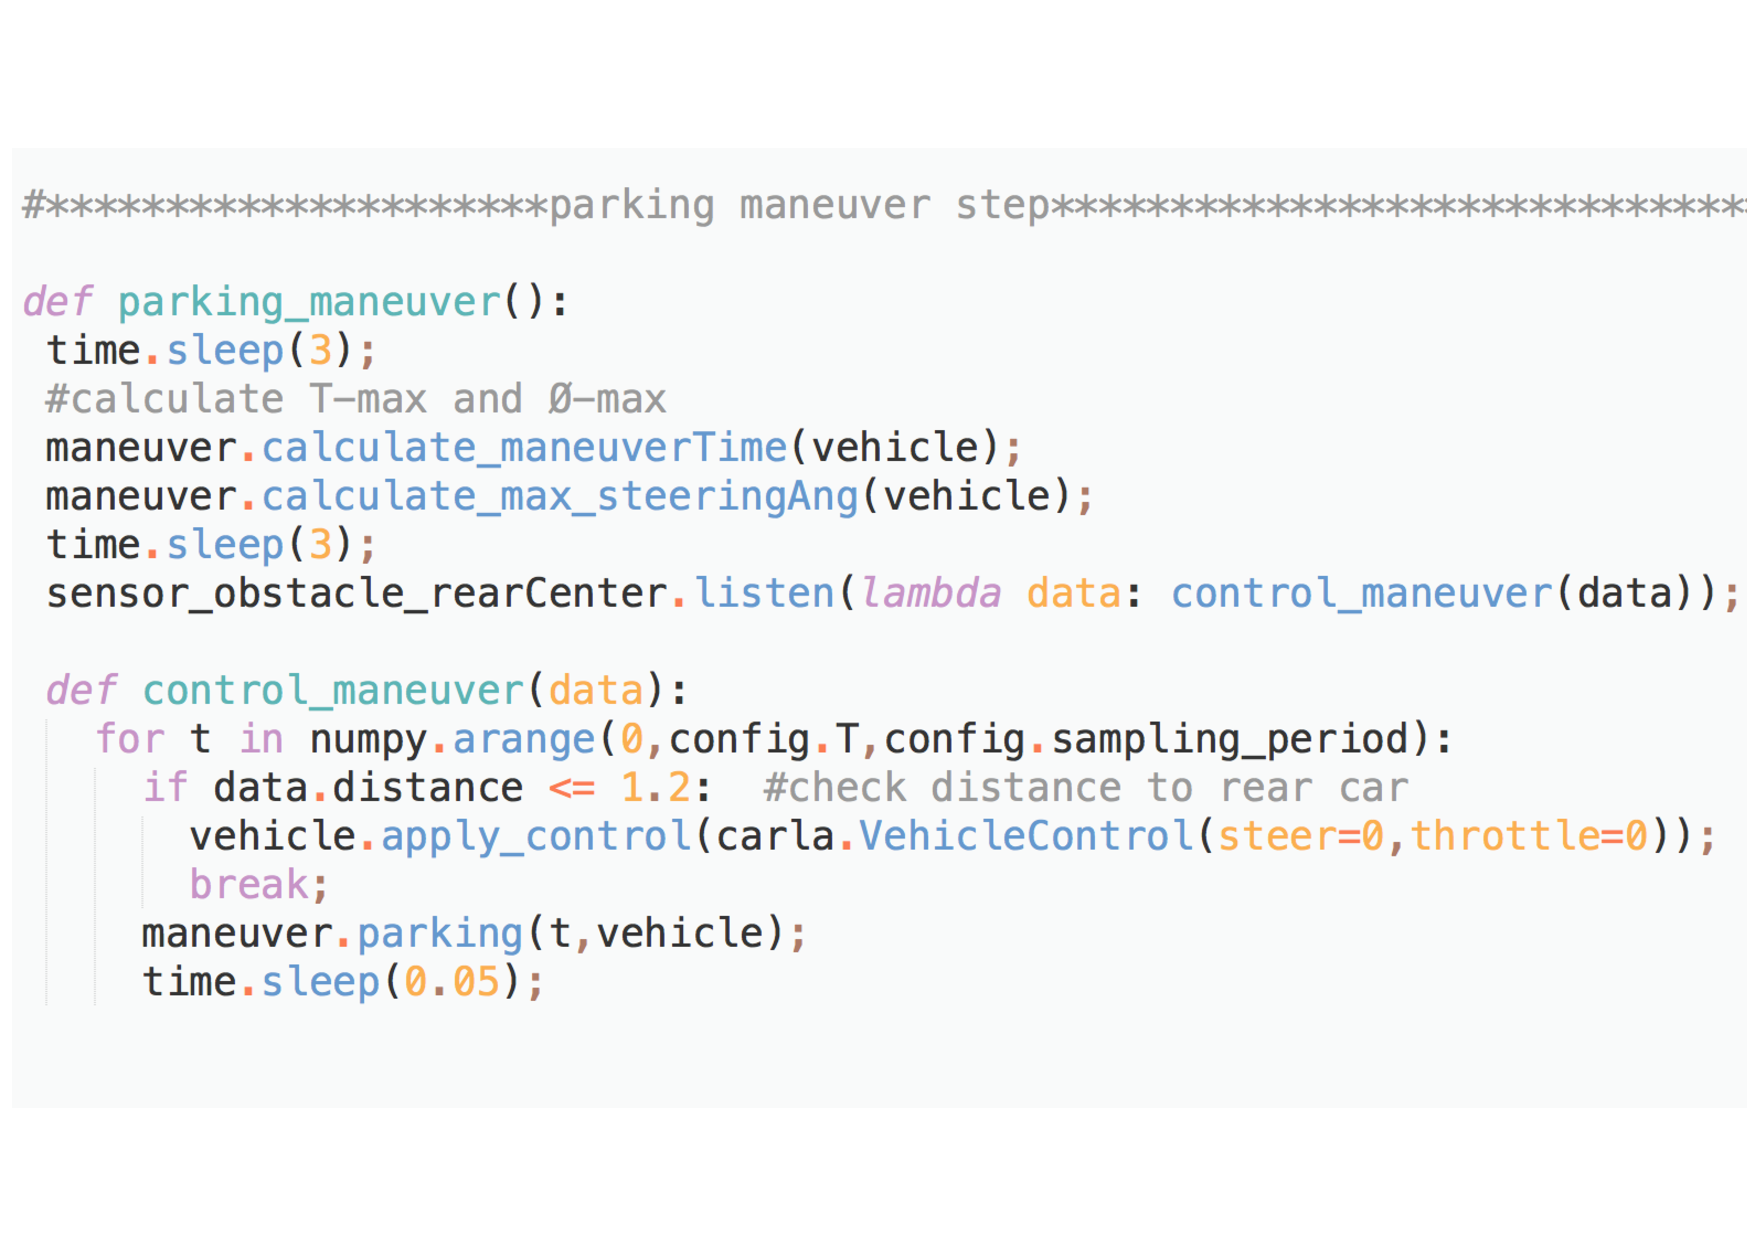
\includegraphics[width=12cm, height=6cm]{images/parkingManeuver.pdf}
    \caption{Parking-maneuver function}
    \label{fig:maneuverCodes}
\end{figure}



As it can be seen in \ref{fig:maneuverCodes}, to control collision, obstacle sensors are used and each time the sensor generates data, another function called control-maneuver() will be called so the distance of vehicle to detected obstacles will be checked in each time stamp and if the distance is considered to be safe, parking function from maneuver.py is executed. Parking() function gets time and also vehicle data as input arguments to set the vehicle's arguments as speed and steering. So maneuver.parking(t, vehicle) access to the steeringAngle(t) and velocity(t) in maneuver.py and each time of simulation, it gets new steering and velocity values and apply this new values to the vehicle. As we can also see from the above codes, end of maneuver depends on the sensor output as this output, when vehicle's distance to rear side is small, ego-vehicle should be stopped and the situation is considered as parked. So the loop will be broken and steering and velocity values will be set to 0 and vehicle will be stopped. 
It is also important to mention that, because of the problem we had in Carla to set velocity values, this value is not set directly and is set through throttle parameter. Because by setting throttle value, velocity of vehicle will be also affected as their values are not independent and also if we just set the velocity by using set-velocity() function in Carla without setting throttle, engines brakes will decrease vehicle velocity \cite{setVelocity}. Fig \ref{fig:velo} shows how the velocity has been set in this implementation. As it can be seen, velocity of vehicle is compared with the expected velocity which we get from velocity(t) function and if it would be higher, an increase is applied to the brake otherwise, throttle would be increased so we set the velocity by controlling the throttle like in real car.
\begin{figure}
\centering
    \includegraphics[width=10cm, height=6cm]{images/velo.pdf} 
    \caption{Set Velocity For Parking Motion}
    \label{fig:velo}
\end{figure}
Time maneuver and phi are defined as global value so they could be accessed by all functions and could be changed during calculation we also needed to define a a maximum value for velocity which should be accessed by velocity(t) function. All of these global and constant values have been defined in config.py file and are accessible with all the other python scripts.
Sampling period of the maneuver simulation should be also defined and all of the calculations are based on this sampling-period. Sampling-period in Carla is adjusted by FPS which is fps rate or sampling rate of simulation. That is also possible to set the fix sampling rate of simulation in Carla and in this project, it is set to -fps 20 in each time of simulation. Every time we perform Carla we should set the parameters $-benchmark -fps 20$ where benchmark means that simulation will be in a fix sampling rate and fps 20 means that simulation is in every 0.05s (seconds). Hence, sampling-period of maneuver has been defined to 0.05 in config.py and this value will be used to calculate T$_{max}$ and $\Phi_{max}$. During calculations of time, steering, loops are incremented by this value and in a different sampling rate, maneuver would not be worked or sampling-period in config.py should be changed by changing fps.